% LuaLaTeX

\documentclass[a4paper, twoside, 12pt]{article}
\usepackage[latin]{babel}
%\usepackage[landscape, left=3cm, right=1.5cm, top=2cm, bottom=1cm]{geometry} % okraje stranky
\usepackage[portrait, a4paper, mag=1300, truedimen, left=0.8cm, right=0.8cm, top=0.8cm, bottom=0.8cm]{geometry} % okraje stranky

\usepackage{fontspec}
\setmainfont[FeatureFile={junicode.fea}, Ligatures={Common, TeX}, RawFeature=+fixi]{Junicode}
%\setmainfont{Junicode}

% shortcut for Junicode without ligatures (for the Czech texts)
\newfontfamily\nlfont[FeatureFile={junicode.fea}, Ligatures={Common, TeX}, RawFeature=+fixi]{Junicode}

\usepackage{multicol}
\usepackage{color}
\usepackage{lettrine}
\usepackage{fancyhdr}

% usual packages loading:
\usepackage{luatextra}
\usepackage{graphicx} % support the \includegraphics command and options
\usepackage{gregoriotex} % for gregorio score inclusion
\usepackage{gregoriosyms}
\usepackage{wrapfig} % figures wrapped by the text
\usepackage{parcolumns}
\usepackage[contents={},opacity=1,scale=1,color=black]{background}
\usepackage{tikzpagenodes}
\usepackage[savepos]{zref}
\usepackage{calc}
\usepackage{longtable}
\newif\ifparvulus
\newif\ifsimeon
\newif\ifignatius
\parvulustrue
\ignatiustrue

\setlength{\headheight}{12pt}

% Commands used to produce a typical "Conventus" booklet

\newenvironment{titulusOfficii}{\begin{center}}{\end{center}}
\newcommand{\dies}[1]{#1

}
\newcommand{\nomenFesti}[1]{\textbf{\Large #1}

}
\newcommand{\celebratio}[1]{#1

}

\newcommand{\hora}[1]{%
\vspace{0.5cm}{\large \textbf{#1}}

\fancyhead[LE]{\thepage\ / #1}
\fancyhead[RO]{#1 / \thepage}
\addcontentsline{toc}{subsection}{#1}
}

% larger unit than a hora
\newcommand{\divisio}[1]{%
\begin{center}
{\Large \textsc{#1}}
\end{center}
\fancyhead[CO,CE]{#1}
\addcontentsline{toc}{section}{#1}
}

% a part of a hora, larger than pars
\newcommand{\subhora}[1]{
\begin{center}
{\large \textit{#1}}
\end{center}
%\fancyhead[CO,CE]{#1}
\addcontentsline{toc}{subsubsection}{#1}
}

% rubricated inline text
\newcommand{\rubricatum}[1]{\textit{#1}}

% standalone rubric
\newcommand{\rubrica}[1]{\vspace{3mm}\rubricatum{#1}}

\newcommand{\notitia}[1]{\textcolor{red}{#1}}

\newcommand{\scriptura}[1]{\hfill \small\textit{#1}}

\newcommand{\translatioCantus}[1]{\vspace{1mm}%
{\noindent\footnotesize \nlfont{#1}}}

% pruznejsi varianta nasledujiciho - umoznuje nastavit sirku sloupce
% s prekladem
\newcommand{\psalmusEtTranslatioB}[3]{
  \vspace{0.5cm}
  \begin{parcolumns}[colwidths={2=#3}, nofirstindent=true]{2}
    \colchunk{
      \input{#1}
    }

    \colchunk{
      \vspace{-0.5cm}
      {\footnotesize \nlfont
        \input{#2}
      }
    }
  \end{parcolumns}
}

\newcommand{\psalmusEtTranslatio}[2]{
  \psalmusEtTranslatioB{#1}{#2}{8.5cm}
}


\newcommand{\canticumMagnificatEtTranslatio}[1]{
  \psalmusEtTranslatioB{#1}{temporalia/extra-adventum-vespers/magnificat-boh.tex}{12cm}
}
\newcommand{\canticumBenedictusEtTranslatio}[1]{
  \psalmusEtTranslatioB{#1}{temporalia/extra-adventum-laudes/benedictus-boh.tex}{10.5cm}
}

% volne misto nad antifonami, kam si zpevaci dokresli neumy
\newcommand{\hicSuntNeumae}{\vspace{0.5cm}}

% prepinani mista mezi notovymi osnovami: pro neumovane a neneumovane zpevy
\newcommand{\cantusCumNeumis}{
  \setgrefactor{17}
  \global\advance\grespaceabovelines by 5mm%
}
\newcommand{\cantusSineNeumas}{
  \setgrefactor{17}
  \global\advance\grespaceabovelines by -5mm%
}

% znaky k umisteni nad inicialu zpevu
\newcommand{\superInitialam}[1]{\gresetfirstlineaboveinitial{\small {\textbf{#1}}}{\small {\textbf{#1}}}}

% pars officii, i.e. "oratio", ...
\newcommand{\pars}[1]{\textbf{#1}}

\newenvironment{psalmus}{
  \setlength{\parindent}{0pt}
  \setlength{\parskip}{5pt}
}{
  \setlength{\parindent}{10pt}
  \setlength{\parskip}{10pt}
}

%%%% Prejmenovat na latinske:
\newcommand{\nadpisZalmu}[1]{
  \hspace{2cm}\textbf{#1}\vspace{2mm}%
  \nopagebreak%

}

% mode, score, translation
\newcommand{\antiphona}[3]{%
\hicSuntNeumae
\superInitialam{#1}
\includescore{#2}

#3
}
 % Often used macros
%%%% Preklady jednotlivych zpevu (nektere se opakuji, a je dobre mit je
% vsechny na jedne hromade)

\newcommand{\trIntroitus}{\translatioCantus{Vous tous qui avez soif,~\grestar{}
venez aux eaux, dit le Seigneur, et vous qui n’avez point d’argent, venez et buvez avec joie.
\textit{\color{red}Ps.} Mon peuple, écoutez ma loi, prêtez l’oreille aux paroles de ma bouche.}}

\newcommand{\trAlleluia}{\translatioCantus{Alleluia. \Vbardot{}
Le Seigneur comme au Sinaï, dans son sanctuaire, est monté au ciel, emmenant
captive notre captivité.}}

\newcommand{\trCommunio}{\translatioCantus{Vous qui avez été baptizés
dans le Christ, vous avez revêtu le Christ~; alleluia~! \Vbardot{}
La voix de l’Eternel retentit sur les eaux,
Dieu, dans sa gloire, fait gronder le tonnerre.~\grestar{}
La voix de l’Eternel domine le bruit des grandes eaux.}}

\newcommand{\trAdorna}{\translatioCantus{
Orne ta chambre nuptiale, Sion, pour y recevoir ton roi, le Christ ;
attache-toi à Marie : elle est la porte du ciel : c'est elle qui porte le
roi de gloire, la lumière nouvelle ; elle reste vierge, elle qui tient
entre ses mains ce Fils né dans l'étoile du matin ; Syméon le reçut dans ses
bras, et annonça aux peuples qu'il est le Seigneur de la vie et de la mort
et le Sauveur du monde.}}

\newcommand{\trSenex}{\translatioCantus{Le vieillard portait l'enfant, mais l'enfant dirigeait le
vieillard.}}

\newcommand{\trLumen}{\translatioCantus{Lumière qui se révèle aux nations et donne gloire à Israël, ton peuple.
Maintenant, Seigneur, tu laisses ton serviteur S’en aller en paix, selon ta
parole. Car mes yeux ont vu ton salut, Salut que tu as préparé devant tous
les peuples, Lumière pour éclairer les nations, Et gloire d’Israël, ton
peuple.»}}

\newcommand{\trDaPacem}{\translatioCantus{Donne la paix, Seigneur, en nos
jours, car il n'y a personne d'autre qui combat pour nous que toi, notre
Dieu.}}
 % Czech translations of the proper texts

\setlength{\columnsep}{15pt} % prostor mezi sloupci

\makeatletter
\newcounter{litscore}
\newcounter{littabstop}[litscore]
\newcommand{\grealign}{%
	\@bsphack%
	\ifgre@boxing\else%
		\kern\gre@dimen@begindifference%
		\stepcounter{littabstop}%
		\expandafter\zsavepos{stop-\thelitscore-\thelittabstop}%
		\kern-\gre@dimen@begindifference%
	\fi%
	\@esphack%
}

\newcommand{\litsetstops}{%
  \gdef\nstabbing@stops{%
    \hspace*{-\oddsidemargin}\hspace{-1in}%
    \hspace*{\zposx{stop-\thelitscore-1} sp}\=%
  }%
  \count@=\@ne
  \loop\ifnum\count@<\value{littabstop}%
    \begingroup\edef\x{\endgroup
      \noexpand\g@addto@macro\noexpand\nstabbing@stops{%
        \noexpand\hspace{-\noexpand\zposx{stop-\thelitscore-\the\count@} sp}%
        \noexpand\hspace{\noexpand\zposx{stop-\thelitscore-\the\numexpr\count@+1} sp}\noexpand\=%
      }%
    }\x
    \advance\count@\@ne
  \repeat
  \nstabbing@stops\kill
}
\makeatother

\newenvironment{nstabbing}
  {\setlength{\topsep}{0pt}%
   \setlength{\partopsep}{0pt}%
   \tabbing%
   \litsetstops}
  {\endtabbing\stepcounter{litscore}}

\renewcommand{\rubricatum}[1]{\textit{\color{red}#1}}

%%%%%%%%%%%%%%%%%%%%%%%%%%%%%%%%%%%%%%%%%%%%%%%%%%%%%%%%%%%%%%%%%%%%%%%%%%%%%%%%%%%%%%%%%%%%%%%%%%%%%%%%%%%%%
\begin{document}

% Here we set the space around the initial.
% Please report to http://home.gna.org/gregorio/gregoriotex/details for more details and options
\grechangedim{afterinitialshift}{2.2mm}{scalable}
\grechangedim{beforeinitialshift}{2.2mm}{scalable}
\grechangedim{interwordspacetext}{0.20 cm plus 0.15 cm minus 0.05 cm}{scalable}%
\grechangedim{annotationraise}{-0.2cm}{scalable}

% Here we set the initial font. Change 38 if you want a bigger initial.
% Emit the initials in red.
\grechangestyle{initial}{\color{red}\fontsize{38}{38}\selectfont}

\renewcommand{\headrulewidth}{0pt} % no horiz. rule at the header
\pagestyle{empty}

\grechangedim{spaceabovelines}{0.2cm}{scalable}%

\begin{center}
{\LARGE ORDO BAPTISMI PARVULORUM}

\vspace{0.5cm}

\ifparvulus
\ifignatius
{\Large Ignatius Ludovicus Srovnal\\
26. Augusti MMXXII}
\else
\ifsimeon
{\Large Simeon Rochus Srovnal\\
25. Iulii MMXXI}
\else
{\Large Angelus Benedictus-Ioseph Srovnal\\
19. Ianuarii MMXIX}
\fi
\fi
\else
{\Large Myrrha Liesse Srovnalová\\
18. Februarii MMXVII}
\fi

\vspace{1cm}

\ifparvulus
\ifignatius
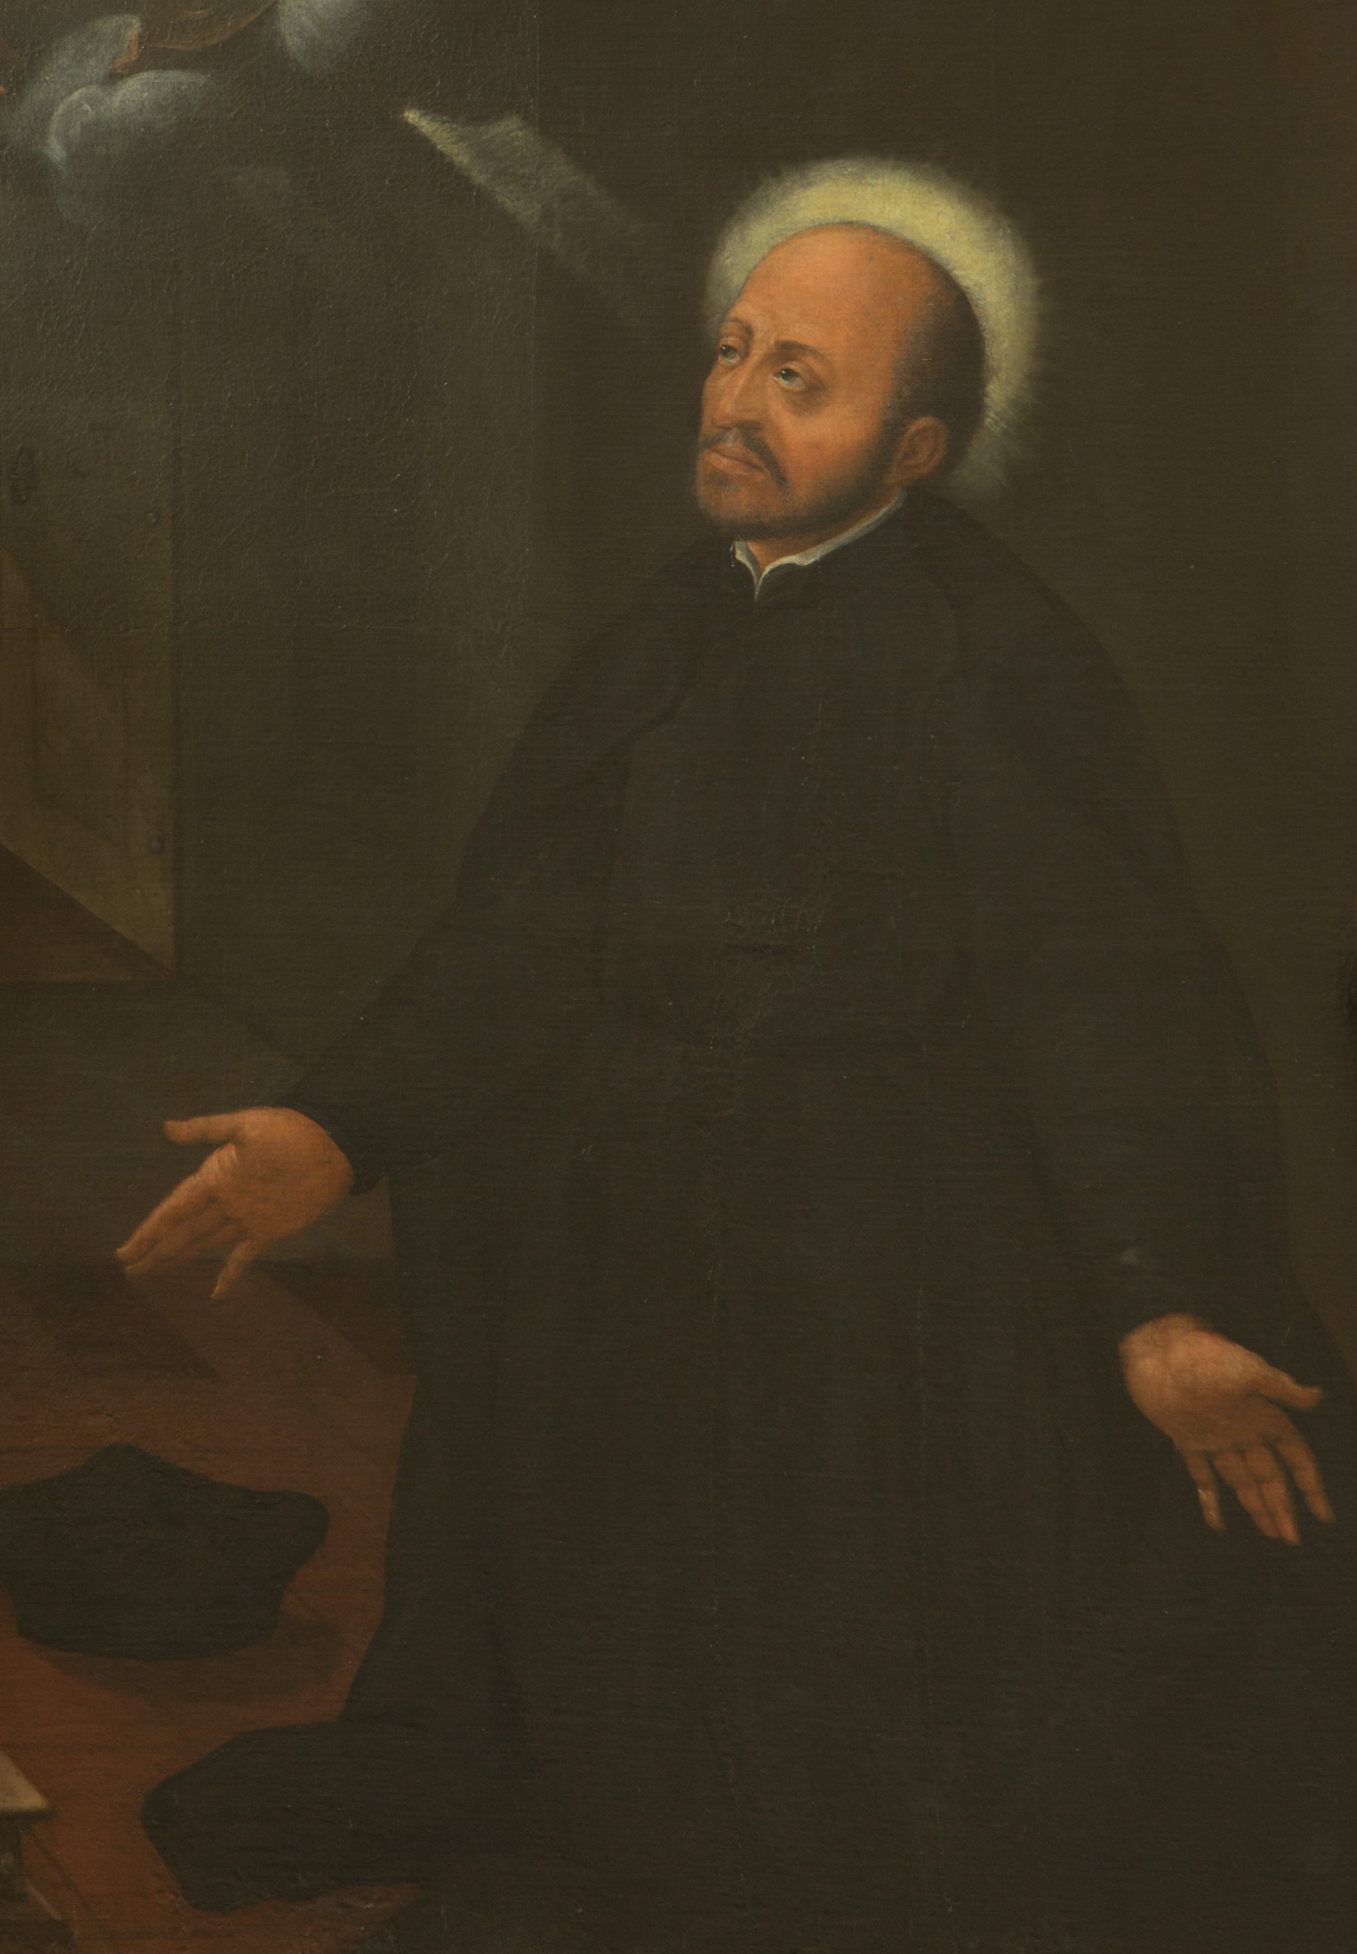
\includegraphics[width=5cm]{ignatius.jpg}
\else
\ifsimeon
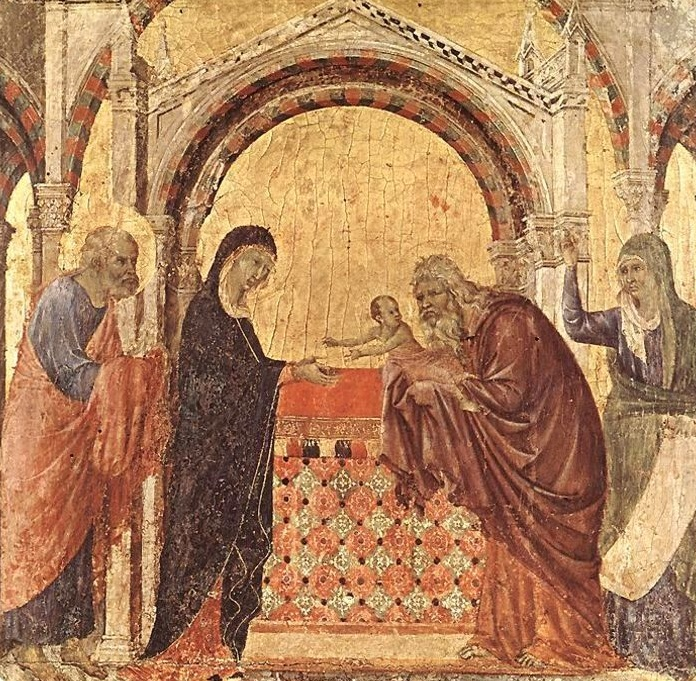
\includegraphics[width=5cm]{siena.jpg}
\else
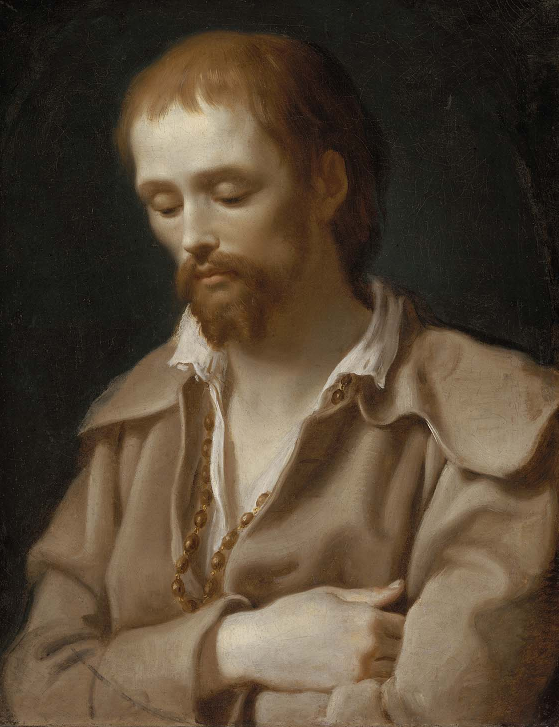
\includegraphics[width=5cm]{benedictlabre.png}
\fi
\else
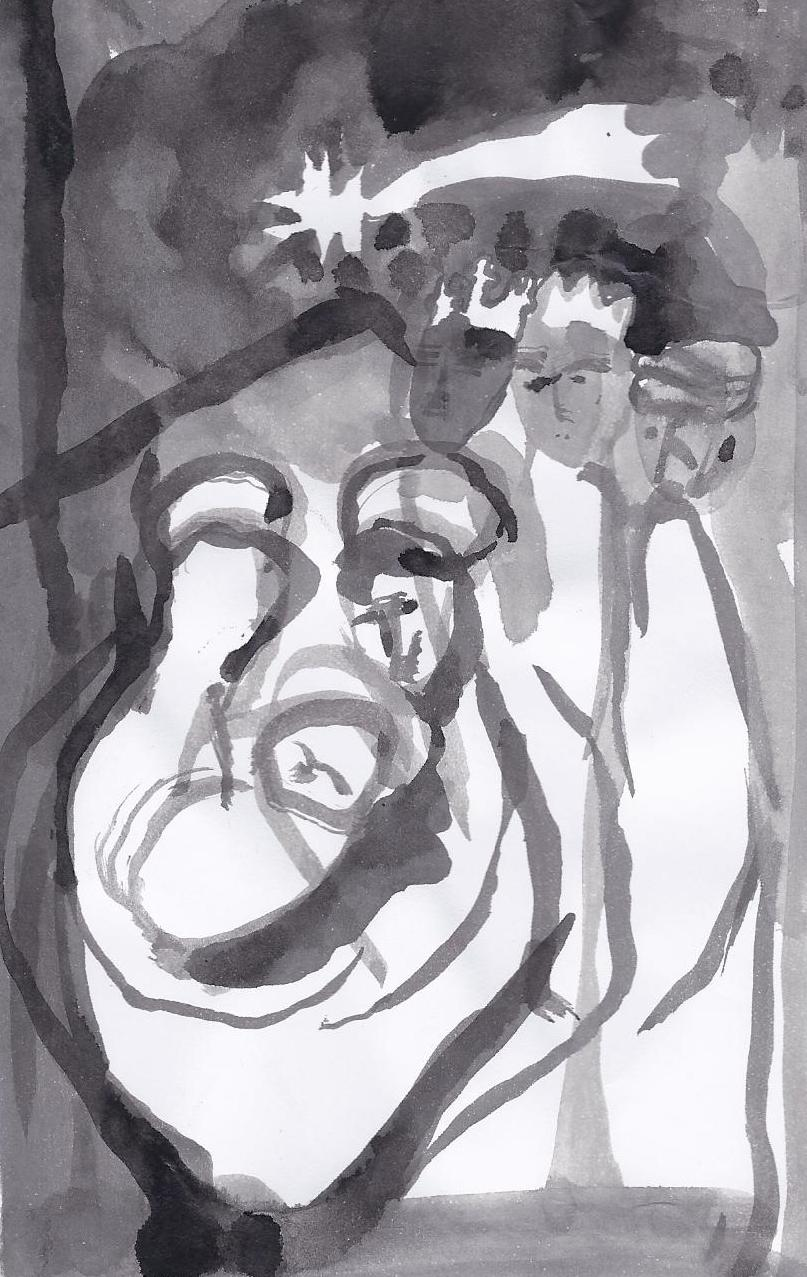
\includegraphics[width=5cm]{ordobaptismi.jpg}
\fi
\fi

\vspace{0.2cm}

\end{center}

\vfill

\ifsimeon
\vfill
\else
\gresetnabcfont{grelaon}{8}

\pars{Antiphona ad introitum} \scriptura{Cf. Is. 55, 1; Ps. 77, 1; \textbf{L75}}

\vspace{-0.6cm}

\antiphona{II}{temporalia/introitus-Sitientes.gtex}

\trIntroitus

\vfill
\pagebreak
\fi

\pars{\textsc{Ritus recipiendi parvulum}}

\vspace{-0.3cm}

\psalmusEtTranslatioT{temporalia/ritusrecipiendi-combfr.tex}{6cm}

\ifsimeon
\pars{\textsc{Antiphona}} \scriptura{E72}

\antiphona{VI}{temporalia/ant-adornathalamum.gtex}

\trAdorna

\vfill
\pagebreak
\fi

\ifignatius
\pars{\textsc{Ad processionem}}

\gresetnabcfont{gregall}{8}

\antiphona{VI}{temporalia/alleluia.gtex}

\scriptura{Ps. 117, 1-6}

\initiumpsalmi{temporalia/communio-versus-Confitemini-initium.gtex}

\vspace{-1cm}

\psalmusEtTranslatioTS{temporalia/communio-versus-Confitemini-combfr.tex}{6cm}

\pars{\textsc{Sacra verbi Dei celebratio}}

\pars{Graduale}

\psalmusEtTranslatioT{temporalia/graduale-combfr.tex}{6cm}
\else
\pars{\textsc{Sacra verbi Dei celebratio}}

\gresetnabcfont{gregall}{8}

\ifsimeon
\pars{Alleluia}

\vspace{-0.3cm}

\antiphona{I}{temporalia/alleluia-SenexPuerum.gtex}

\trSenex

\vspace{-0.3cm}

\else
\pars{Alleluia} \scriptura{Ps. 67, 18.19; \textbf{C116}}

\vspace{-0.6cm}

\antiphona{VIII}{temporalia/alleluia-DominusInSina.gtex}

\vspace{-0.3cm}

\trAlleluia
\fi
\fi

\gresetnabcfont{grelaon}{8}

\vspace{-0.3cm}

\psalmusEtTranslatioT{temporalia/evangelium-initium-combfr.tex}{6cm}

\vspace{-0.2cm}

\ifparvulus
\ifsimeon
\pars{Léctio sancti Evángelii secúndum Lucam.} \scriptura{Lc. 2, 22-40}

%\vspace{-0.2cm}

%\psalmusEtTranslatioT{temporalia/evangelium3-combfr.tex}{6cm}
\rubricatum{\Rbardot{}} Gloire à toi, Seigneur.

Quand fut arrivé le huitième jour, celui de la circoncision, l'enfant reçut
le nom de Jésus, le nom que l'ange lui avait donné avant sa conception.
Quand arriva le jour fixé par la loi de Moïse pour la purification, les
parents de Jésus le portèrent à Jérusalem pour le présenter au Seigneur,
selon ce qui est écrit dans la Loi : Tout premier-né de sexe masculin sera
consacré au Seigneur. Ils venaient aussi présenter en offrande le sacrifice
prescrit par la loi du Seigneur : un couple de tourterelles ou deux petites
colombes. Or, il y avait à Jérusalem un homme appelé Syméon. C'était un
homme juste et religieux, qui attendait la consolation d'Israël, et
l'Esprit Saint était sur lui. L'Esprit lui avait révélé qu'il ne verrait
pas la mort avant d'avoir vu le Messie du Seigneur. Poussé par l'Esprit,
Syméon vint au Temple. Les parents y entraient avec l'enfant Jésus pour
accomplir les rites de la Loi qui le concernaient. Syméon prit l'enfant
dans ses bras, et il bénit Dieu en disant : « Maintenant, ô Maître, tu peux
laisser ton serviteur s'en aller dans la paix, selon ta parole. Car mes
yeux ont vu ton salut, que tu as préparé à la face de tous les peuples :
lumière pour éclairer les nations païennes, et gloire d'Israël ton peuple.
» Le père et la mère de l'enfant s'étonnaient de ce qu'on disait de lui.
Syméon les bénit, puis il dit à Marie sa mère : « Vois, ton fils qui est là
provoquera la chute et le relèvement de beaucoup en Israël. Il sera un
signe de division. — Et toi-même, ton cœur sera transpercé par une épée. —
Ainsi seront dévoilées les pensées secrètes d'un grand nombre. » Il y avait
là une femme qui était prophète, Anne, fille de Phanuel, de la tribu
d'Aser. Demeurée veuve après sept ans de mariage, elle avait atteint l'âge
de quatre-vingt-quatre ans. Elle ne s'éloignait pas du Temple, servant Dieu
jour et nuit dans le jeûne et la prière. S'approchant d'eux à ce moment,
elle proclamait les louanges de Dieu et parlait de l'enfant à tous ceux qui
attendaient la délivrance de Jérusalem. Lorsqu'ils eurent accompli tout ce
que prescrivait la loi du Seigneur, ils retournèrent en Galilée, dans leur
ville de Nazareth. L'enfant grandissait et se fortifiait, tout rempli de
sagesse, et la grâce de Dieu était sur lui.

Acclamons la Parole de Dieu.

\rubricatum{\Rbardot{}} Louange à toi, Seigneur Jésus.


\vspace{0.2cm}
\else
\pars{Léctio sancti Evángelii secúndum Marcum.} \scriptura{Mc. 10, 13-16}

\vspace{-0.2cm}

\psalmusEtTranslatioT{temporalia/evangelium2-combfr.tex}{6cm}
\fi
\else
\pars{Léctio sancti Evángelii secúndum Ioánnem.} \scriptura{Io. 19, 38-42}

\vspace{-0.2cm}

\psalmusEtTranslatioT{temporalia/evangelium-combfr.tex}{6cm}
\fi

\vspace{-0.2cm}

\ifignatius
\pars{Hymnus}

\antiphona{VIII}{temporalia/hym-VeniCreator.gtex}

\vspace{0.3cm}

\vfill
\pagebreak
\else
\ifsimeon
\pars{Hymnus}

\antiphona{VIII}{temporalia/hym-VeniCreator.gtex}

\vspace{0.3cm}
\fi
\fi

\noindent\pars{Oratio fidelium}

\vspace{-0.5cm}

\psalmusEtTranslatioT{temporalia/oratiofidelium-combfr.tex}{6cm}

\sineinitiali{temporalia/terogamus.gtex}

\psalmusEtTranslatioT{temporalia/oratiofidelium-2-combfr.tex}{6cm}

\sineinitiali{temporalia/litaniae.gtex}

\begin{nstabbing}
\ifparvulus
\>Sancti Angeli \>\>\>\>\textbf{De}-\>\>i, \>orá-\>\>\textit{te} \>\textit{pro} \textbf{no}bis.\\
\fi
\>Sancte Ioánnes \>\>\>Ba-\textbf{ptí}-\>\>\>sta, \>\>o-\>\textit{ra} \>\textit{pro} \textbf{no}bis.\\
\>Sancte \>\>\>\>\textbf{Io}-\>seph, \>\>\>o-\>\textit{ra} \>\textit{pro} \textbf{no}bis.\\
\>Sancti Petre et \>\>\>\>\textbf{Pau}-\>\>le, \>orá-\>\>\textit{te} \>\textit{pro} \textbf{no}bis.\\
\textellipsis
\end{nstabbing}

\noindent\pars{Oratio exorcismi et uncio præbaptismalis}

\vspace{-0.3cm}

\psalmusEtTranslatioT{temporalia/exorcismus-combfr.tex}{6cm}

\pars{\textsc{Celebratio baptismi}}

\vspace{-0.3cm}

\psalmusEtTranslatioT{temporalia/celebratio-baptismi-combfr.tex}{6cm}

\pars{\textsc{Ritus explanativi}}

\vspace{-0.3cm}

\psalmusEtTranslatioT{temporalia/ritus-explanativi-combfr.tex}{6cm}

\pars{\textsc{Conclusio ritus}}

\vspace{-0.5cm}

\ifsimeon
\scriptura{Lc. 2, 32; \textbf{H120}}

\vspace{-4mm}

\antiphona{VIII a}{temporalia/ant-lumenadrevelationem.gtex}

\trLumen
\else
\scriptura{Gal. 3, 27; \textbf{L112}}

\vspace{-0.6cm}

\antiphona{II}{temporalia/communio-OmnesQui.gtex}
\fi

\ifparvulus
\ifsimeon
\else
\scriptura{Ps. 28, 3}

\initiumpsalmi{temporalia/communio-versus-Vox-initium.gtex}
\fi
\fi

\ifsimeon
\else
\trCommunio
\fi

\vspace{-0.3cm}

\psalmusEtTranslatioT{temporalia/conclusio-ritus-combfr.tex}{6cm}

\vfill

\vspace{-0.3cm}

\ifparvulus
\ifignatius
\gresetnabcfont{gregall}{8}

\pars{Pro pace in Ucraina.} \scriptura{Sir. 50, 25; 2 Esdr. 4, 20; \textbf{H416}}

\vspace{-4mm}

\antiphona{II D}{temporalia/ant-dapacemdomine.gtex}

\trDaPacem

\vfill
\pagebreak

\pars{Antiphona B.M.V.}

\antiphona{I}{temporalia/an_salve_regina.gtex}
\else
\ifsimeon
\antiphona{V}{temporalia/ant-salveregina-simplex.gtex}

\antiphona{VI}{temporalia/alleluia.gtex}

\scriptura{Ps. 117, 1-6}

\initiumpsalmi{temporalia/communio-versus-Confitemini-initium.gtex}

\vspace{-1cm}

\psalmusEtTranslatioTS{temporalia/communio-versus-Confitemini-combfr.tex}{6cm}
\else
\vspace{-0.3cm}
\antiphona{}{temporalia/svatyvaclave.gtex}
\fi
\fi
\else
\antiphona{VI}{temporalia/alleluia.gtex}

\scriptura{Ps. 117, 1-6}

\initiumpsalmi{temporalia/communio-versus-Confitemini-initium.gtex}

\vspace{-1cm}

\psalmusEtTranslatioTS{temporalia/communio-versus-Confitemini-combfr.tex}{6cm}
\fi

\vfill

\end{document}
